\chapter{Term Lister}\label{chap:lister}

When I was strenuously writing my Pāli books, this tool was one of the most used. Now it has capability to handle all text collections, thanks to Lucene. In early versions of the program, this tool used pre-built term lists. Now it uses term/token lists from indexes created by Lucene Finder. This means, essentially, you have to know how to build an index from a text collection first (see Chapter \ref{chap:lucene}). Once you have an index of the collection, you can explore its term list.

\dothis{To use Term Lister, click {\faSix \symbol{"F0CA}} button on the main tool bar, or use menu Lucene > {\faSix \symbol{"F0CA}} Term Lister. Or you can use its tab in the main window by loading the tool when needed.\\
\hspace{5mm}Before using Term Lister, create an index from a text collection with Lucene Finder first.
}

Even if you have an index, you cannot use the tool right away. You have to build a lister table from that index before you can see the list.

\section{How to build a lister table}

Figure \ref{fig:lister-empty} shows Term Lister at the first run before any table is created. The empty selector means the tool is not ready yet. The next thing to do, if you have already created some indexes with Lucene Finder, is opening the listing options by hitting {\faSix \symbol{"F085}} button. If an index is available, you can see its name in the index selector with a short description (see the picture). Select the index you need and consider whether you want to include terms in notes or not. For more information about text fields, see Section \ref{sect:textfields} on page \pageref{sect:textfields}. Remember that not all collections have notes in their texts.

\begin{figure}[!hbt]
\centering
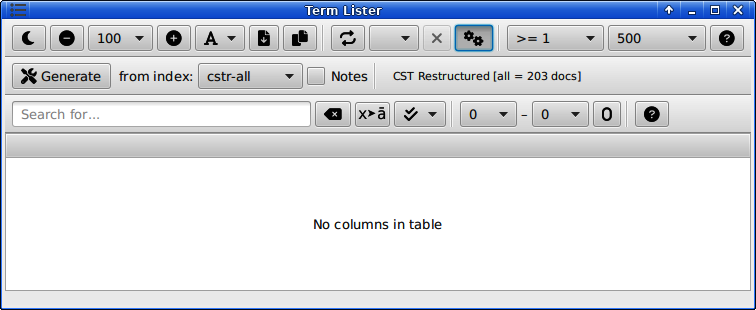
\includegraphics[width=0.9\linewidth]{images/lister-empty.png}\\
\caption{Term Lister in the first run with listing options opened}
\label{fig:lister-empty}
\end{figure}

When you are satisfied with the listing options, then hit {\faSix \symbol{"F7D9}} Generate button and wait a minute (maybe shorter or longer depending on the index's size). Once the creation is done, you will have the table's name in the top selector. When this table is selected, its content will show in the table area below (see Figure \ref{fig:lister-table}).

\boxnote{The name of a lister table created is automatically set according to its source index and options. The abbreviations are intuitive and easily recognizable, but you may have to get familiar with the system.}

\dothis{After all needed lister tables are created, it is a good practice to lock the Lister database by toggling this menu:\\
\menucommand{Lucene > {\faSix \symbol{"F09C}} Lister DB unlocked}\\
to\\
\menucommand{Lucene > {\faSix \symbol{"F023}} Lister DB locked}\\
\\
Now then the listing options will be disabled.
}

\begin{figure}[!hbt]
\centering
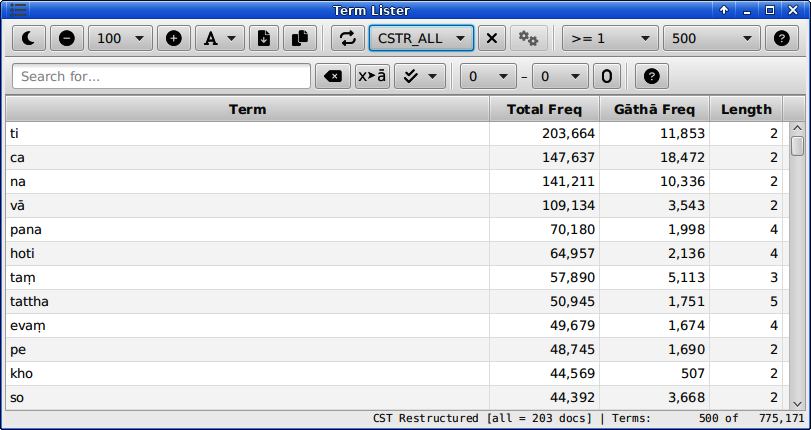
\includegraphics[width=0.9\linewidth]{images/lister-table.png}\\
\caption{Term Lister when a table is available}
\label{fig:lister-table}
\end{figure}

If you are not satisfied with the table created, like you may have forgotten to include notes, for example, you can delete the table with {\faSix \symbol{"F00D}} button and create it again. If you feel that the table selector is not updated, press {\faSix \symbol{"F363}} (Refresh) button.

\section{The result table and displaying options explained}

The result table of Term Lister is made simple by design. It may have three or four columns depending on whether the collection have fields marked as gāthā (verse) or not. In the example above, the result of CSTR collection has four columns: (1) term, (2) total frequency, (3) gāthā frequency, and (4) term's length.

What counted as `term' here is simply a token. It is not a Pāli word in strict sense. A token, in the domain of computational Pāli, is a chunk of character string without in-between separators. So, a portion with punctuation marks will be split with those marks resulting in standalone tokens. The tokenization process is done by indexing (Lucene Finder). All tokens are also normalized into lowercase letters.\footnote{Unlike early versions of the program, the option of keeping capitalized terms is now removed. Because I found that in CSTR collection (the former CSCD) the capitalization was somewhat incomplete or not good enough for analyses. Moreover, I prefer making and using uncapitalized text collections.}

The term's total frequency is the number of occurrences found totally in the documents indexed, including in verse (gāthā) form. The gāthā frequency is the term's occurrences present in verses (if gāthā's related fields available). The gāthā frequency can give you some insight about the word's uses. For example, if a term has high gāthā frequency relative to the total frequency (say, 90\%), it may be a remnant of the past in an archaic form.

The length of term in the last column is Pāli-sensitive, meaning \pali{th}, for example, has 1 character long. So, you see \pali{tattha} in the list has length = 5.

By default, the result is retrieved only 500 rows, ordered by top frequencies. This can quicken the starting time. You can set the number of maximum rows by the last drop-down option in the tool bar, ranging from 50 to 1,000,000 rows. The less you select the faster you get the result.

The table can be sorted by a specific column by clicking the column header. But remember that the sorting is done only on the existing data limited by the maximum rows chosen. It does not retrieve new data.

\newpage
\boxnote{The result table can be sorted otherwise by clicking the column header.\\
\hspace{5mm}\caveat Sorting the table is done only on the existing data limited by the maximum rows chosen. No new data is fetched.
}

Another useful option is frequency range, the drop-down before the maximum-rows option. By default it is set to \textbf{>=\,1} (greater or equal to 1), meaning all in the range. You can select other criteria to see only what you are interested in. For example, by selecting \textbf{=\,1} (equal to 1) you will see only terms that appear only once. Figure \ref{fig:lister-range-once} shows the result of this selection.

\begin{figure}[!hbt]
\centering
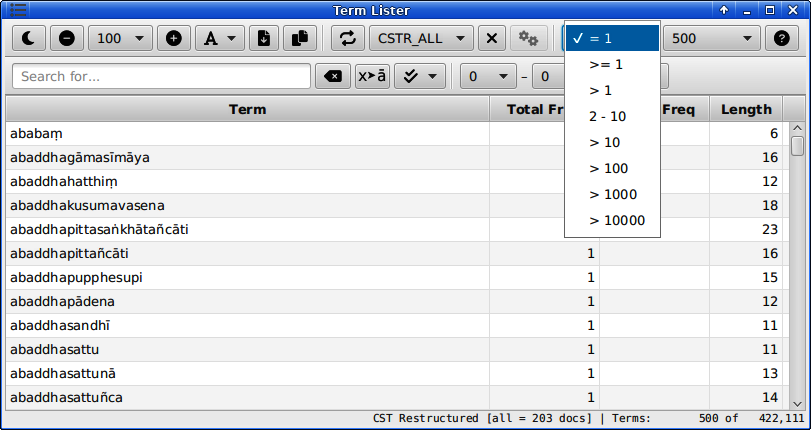
\includegraphics[width=0.9\linewidth]{images/lister-range-once.png}\\
\caption{Terms with frequency = 1 in CSTR}
\label{fig:lister-range-once}
\end{figure}

Now you can apply the options mentioned to find the longest term in a collection. Once you have the target collection and load its table, select 1000000 maximum rows to retrieve all the data. When the result is shown, click the header of column \texttt{Length} twice. (In the first time, it is sorted ascendingly, in the second descendingly.) Figure \ref{fig:lister-toplength} shows the result from all documents in CSTR.

\begin{figure}[!hbt]
\centering
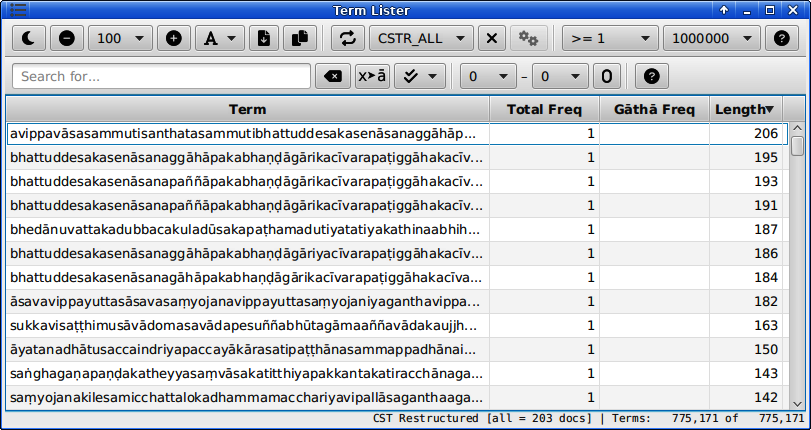
\includegraphics[width=0.9\linewidth]{images/lister-toplength.png}\\
\caption{Top longest terms in CSTR}
\label{fig:lister-toplength}
\end{figure}

If you choose the full frequency range (\textbf{>=\,1}) like me, you have to wait for a big while (around 10 seconds in my old computer). It will be faster if you choose \textbf{=\,1} instead (very long terms are supposed to appear once), because less data will be processed.

You can use a word in the result table or send it to other tools by right-clicking the row you want to open its context menu. Then five choices are available as follows (see their exact wording in Figure \ref{fig:lister-contextmenu}):

\begin{compactenum}[(1)]
\item To copy the word to the system's clipboard
\item To send the word to the main Pāli Dictionaries tab
\item To send the word to the main Sanskrit Dictionaries tab
\item To send the word to the main Document Finder tab
\item To send the word to the main Lucene Finder tab
\end{compactenum}

\dothis{To make use of a term in the lister result, simply drag and drop it to a program's Text Editor opened. Also try dropping elsewhere.\\
\hspace{5mm}To copy the term outside the program, it is better to put it into the system's clipboard first (using context menu).
}

\newpage
\begin{figure}[!hbt]
\centering
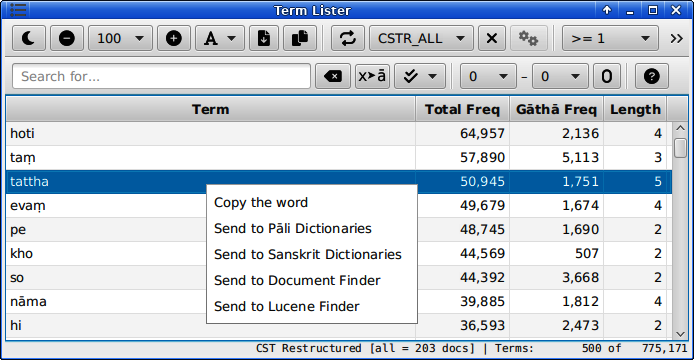
\includegraphics[width=0.9\linewidth]{images/lister-contextmenu.png}\\
\caption{Context menu of the result table}
\label{fig:lister-contextmenu}
\end{figure}

\section{Term filtering strategies}

Term Lister is armed with a powerful search tool that can filter the results in various ways. We have four search modes: (1) Simple filter, (2) Using ? and *, (3) Regular expression, and (4) Filter by meter. These options can be selected by {\faSix \symbol{"F560}} button.

\boxnote{In the first three modes of filtering, the searching is done directly in the database. So, you do not worry that whether your selected maximum-rows is sufficient. In contrast, the meter search is done upon the retrieved data. You have to choose a suitable number of maximum rows.}

\subsection{Simple filtering}

The simplest way to filter the results is selecting by starting letters. When you enter a letter, terms starting with that letter will show up (see Figure \ref{fig:lister-filter-simple}). Entering next characters will refine the filtering further.

\begin{figure}[!hbt]
\centering
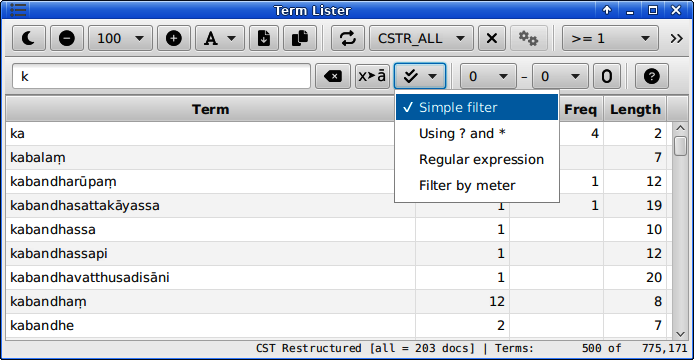
\includegraphics[width=0.9\linewidth]{images/lister-filter-simple.png}\\
\caption{Simple term filtering}
\label{fig:lister-filter-simple}
\end{figure}

\subsection{Filtering by wildcards}

Here, the wildcards, ? (any one character) and * (any number of characters including none), also have their uses, and they are quite helpful if you can figure out how to put them together. See Figure \ref{fig:lister-filter-wildcards} for example.

\begin{figure}[!hbt]
\centering
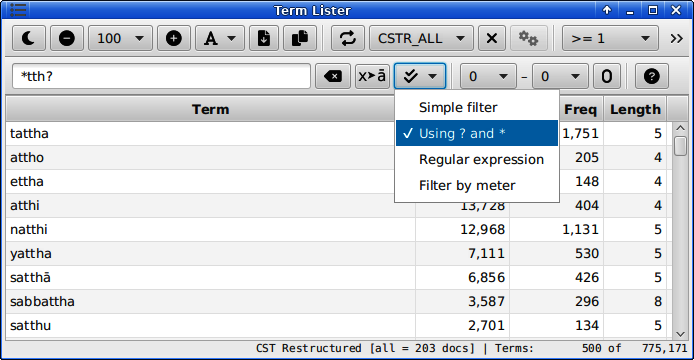
\includegraphics[width=0.9\linewidth]{images/lister-filter-wildcards.png}\\
\caption{Filtering by wildcards}
\label{fig:lister-filter-wildcards}
\end{figure}

\subsection{Filtering by regular expressions}

If you know how to use regular expressions, you can gain a lot of benefits from this mode of filtering. Figure \ref{fig:lister-filter-regexp} shows an example of filtering by a regular expression.\footnote{This is a hit-and-run example to find short words that use \pali{t} or \pali{ṭ} in the second syllable, doubled or not, preceded by \pali{a} and followed by one vowel. You may not have a chance to use this pattern, but it tells you a lot about how regular expression works.} For more information about the syntax, see Chapter \ref{chap:regexp}.

\begin{figure}[!hbt]
\centering
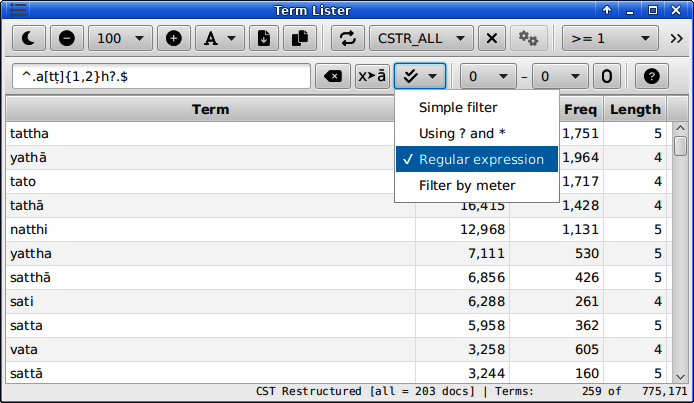
\includegraphics[width=0.9\linewidth]{images/lister-filter-regexp.png}\\
\caption{Filtering by regular expressions}
\label{fig:lister-filter-regexp}
\end{figure}

\subsection{Filtering by prosodic meter}

The last mode of filtering is a kind of fun, but you may not have opportunities to use this often because Pāli prosodic composition is unnecessary nowadays.\footnote{Scholars may see that the topic is too advanced that very few people can master it. Traditional teachers may see this is for only exceptional ones. I see this as an intellectual toy.} When this mode is chosen, the text input symbol will change to musical notes (\texttt{♩♩♪}). Now symbols of meter group, described in Chapter \ref{chap:prosody}, have their corresponding meaning.

The symbols are (case-sensitive) \texttt{1, 2, 4, l, g, n, s, j, b, m, N, S, J, Y, B, R, T, M, } and \texttt{L}.\footnote{The weight \texttt{6} and \texttt{8} are excluded from the process because they are difficult to implement. You have to be specific. For example, using \texttt{24} or \texttt{42} for \texttt{6} and use \texttt{44} for \texttt{8}.} Be careful with \texttt{2} here. It means either \texttt{g} or \texttt{ll}. Figure \ref{fig:lister-filter-meter} (a) shows the result of \texttt{gggl} with 500 terms retrieved, comparing to figure (b), which uses the input \texttt{2221} instead. So, my suggestion is that always use \texttt{g} (not \texttt{2}) when you search with raw meter (\texttt{1} and \texttt{l} bring the same result).

\begin{figure}[!hbt]
\centering
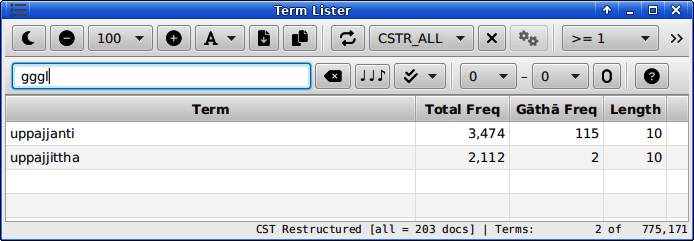
\includegraphics[width=0.9\linewidth]{images/lister-filter-gggl.png}\\
(a) Meter filtering by `gggl'\\[3mm]
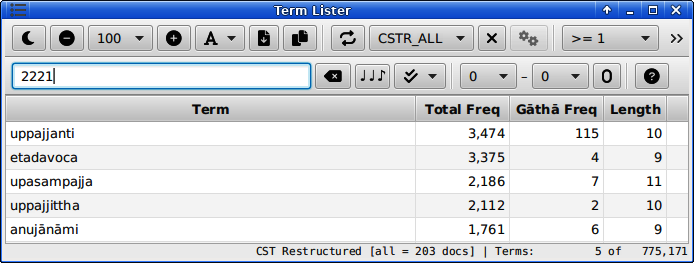
\includegraphics[width=0.9\linewidth]{images/lister-filter-2221.png}\\
(b) Meter filtering by `2221'\\
\caption{Filtering by prosodic meter}
\label{fig:lister-filter-meter}
\end{figure}

\section{Summary by grouping}

The last feature we should know is \emph{grouping}. This can bring us insightfully statistical information. Pāli students may not use this feature often, but it can be useful for textual analyzers or redactors (to find defects, for example). Grouping is an action upon the retrieved data. It groups terms by similarity. For example, you can see that how many terms starting with each letter by setting the start number to 1 (see Figure \ref{fig:lister-grouping-start}). There are some limitations to be aware of. First, characters here are not Pāli-sensitive. This means under the group of `\pali{p-}', for example, terms starting with `\pali{ph-}' are included. And Second, the operation is done upon the existing data, so you have to select a proper number of maximum rows.

\begin{figure}[!hbt]
\centering
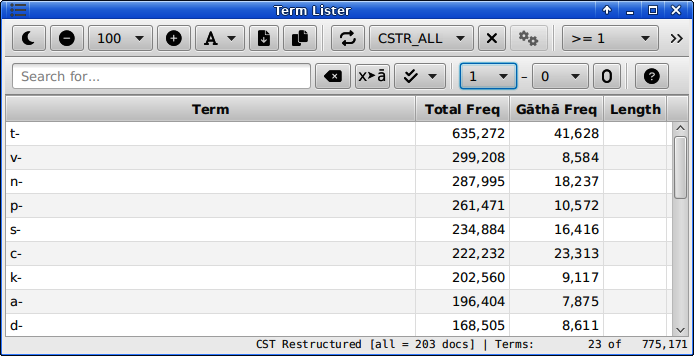
\includegraphics[width=0.9\linewidth]{images/lister-grouping-start.png}\\
\caption{Grouping by the first letter}
\label{fig:lister-grouping-start}
\end{figure}

Similarly, you can see that how many terms ending with the same letters by setting the end number. Figure \ref{fig:lister-grouping-end} shows the result of two-letter endings. Remember that the hyphen (-) includes zero or any number of characters. So, `\pali{-ti}' means `\pali{ti}' itself and everything ending with `\pali{ti}'. You can certainly set both the start and end number to see a particular effect. Please experiment.

\begin{figure}[!hbt]
\centering
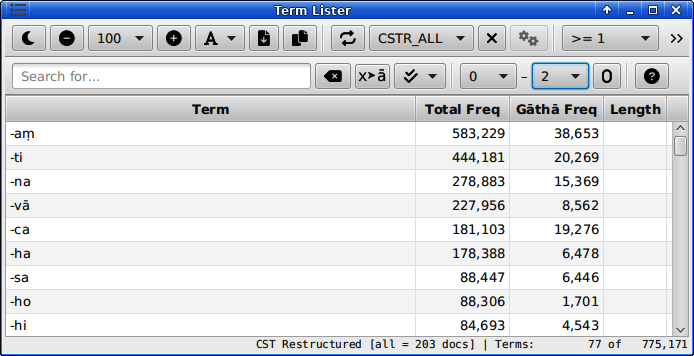
\includegraphics[width=0.9\linewidth]{images/lister-grouping-end.png}\\
\caption{Grouping by the last two letters}
\label{fig:lister-grouping-end}
\end{figure}
